% Options for packages loaded elsewhere
\PassOptionsToPackage{unicode}{hyperref}
\PassOptionsToPackage{hyphens}{url}
%
\documentclass[
]{book}
\usepackage{lmodern}
\usepackage{amssymb,amsmath}
\usepackage{ifxetex,ifluatex}
\ifnum 0\ifxetex 1\fi\ifluatex 1\fi=0 % if pdftex
  \usepackage[T1]{fontenc}
  \usepackage[utf8]{inputenc}
  \usepackage{textcomp} % provide euro and other symbols
\else % if luatex or xetex
  \usepackage{unicode-math}
  \defaultfontfeatures{Scale=MatchLowercase}
  \defaultfontfeatures[\rmfamily]{Ligatures=TeX,Scale=1}
\fi
% Use upquote if available, for straight quotes in verbatim environments
\IfFileExists{upquote.sty}{\usepackage{upquote}}{}
\IfFileExists{microtype.sty}{% use microtype if available
  \usepackage[]{microtype}
  \UseMicrotypeSet[protrusion]{basicmath} % disable protrusion for tt fonts
}{}
\makeatletter
\@ifundefined{KOMAClassName}{% if non-KOMA class
  \IfFileExists{parskip.sty}{%
    \usepackage{parskip}
  }{% else
    \setlength{\parindent}{0pt}
    \setlength{\parskip}{6pt plus 2pt minus 1pt}}
}{% if KOMA class
  \KOMAoptions{parskip=half}}
\makeatother
\usepackage{xcolor}
\IfFileExists{xurl.sty}{\usepackage{xurl}}{} % add URL line breaks if available
\IfFileExists{bookmark.sty}{\usepackage{bookmark}}{\usepackage{hyperref}}
\hypersetup{
  pdftitle={Laboratório de Sistemas de Controle},
  pdfauthor={Djonathan Luiz de Oliveira Quadras},
  hidelinks,
  pdfcreator={LaTeX via pandoc}}
\urlstyle{same} % disable monospaced font for URLs
\usepackage{color}
\usepackage{fancyvrb}
\newcommand{\VerbBar}{|}
\newcommand{\VERB}{\Verb[commandchars=\\\{\}]}
\DefineVerbatimEnvironment{Highlighting}{Verbatim}{commandchars=\\\{\}}
% Add ',fontsize=\small' for more characters per line
\usepackage{framed}
\definecolor{shadecolor}{RGB}{248,248,248}
\newenvironment{Shaded}{\begin{snugshade}}{\end{snugshade}}
\newcommand{\AlertTok}[1]{\textcolor[rgb]{0.94,0.16,0.16}{#1}}
\newcommand{\AnnotationTok}[1]{\textcolor[rgb]{0.56,0.35,0.01}{\textbf{\textit{#1}}}}
\newcommand{\AttributeTok}[1]{\textcolor[rgb]{0.77,0.63,0.00}{#1}}
\newcommand{\BaseNTok}[1]{\textcolor[rgb]{0.00,0.00,0.81}{#1}}
\newcommand{\BuiltInTok}[1]{#1}
\newcommand{\CharTok}[1]{\textcolor[rgb]{0.31,0.60,0.02}{#1}}
\newcommand{\CommentTok}[1]{\textcolor[rgb]{0.56,0.35,0.01}{\textit{#1}}}
\newcommand{\CommentVarTok}[1]{\textcolor[rgb]{0.56,0.35,0.01}{\textbf{\textit{#1}}}}
\newcommand{\ConstantTok}[1]{\textcolor[rgb]{0.00,0.00,0.00}{#1}}
\newcommand{\ControlFlowTok}[1]{\textcolor[rgb]{0.13,0.29,0.53}{\textbf{#1}}}
\newcommand{\DataTypeTok}[1]{\textcolor[rgb]{0.13,0.29,0.53}{#1}}
\newcommand{\DecValTok}[1]{\textcolor[rgb]{0.00,0.00,0.81}{#1}}
\newcommand{\DocumentationTok}[1]{\textcolor[rgb]{0.56,0.35,0.01}{\textbf{\textit{#1}}}}
\newcommand{\ErrorTok}[1]{\textcolor[rgb]{0.64,0.00,0.00}{\textbf{#1}}}
\newcommand{\ExtensionTok}[1]{#1}
\newcommand{\FloatTok}[1]{\textcolor[rgb]{0.00,0.00,0.81}{#1}}
\newcommand{\FunctionTok}[1]{\textcolor[rgb]{0.00,0.00,0.00}{#1}}
\newcommand{\ImportTok}[1]{#1}
\newcommand{\InformationTok}[1]{\textcolor[rgb]{0.56,0.35,0.01}{\textbf{\textit{#1}}}}
\newcommand{\KeywordTok}[1]{\textcolor[rgb]{0.13,0.29,0.53}{\textbf{#1}}}
\newcommand{\NormalTok}[1]{#1}
\newcommand{\OperatorTok}[1]{\textcolor[rgb]{0.81,0.36,0.00}{\textbf{#1}}}
\newcommand{\OtherTok}[1]{\textcolor[rgb]{0.56,0.35,0.01}{#1}}
\newcommand{\PreprocessorTok}[1]{\textcolor[rgb]{0.56,0.35,0.01}{\textit{#1}}}
\newcommand{\RegionMarkerTok}[1]{#1}
\newcommand{\SpecialCharTok}[1]{\textcolor[rgb]{0.00,0.00,0.00}{#1}}
\newcommand{\SpecialStringTok}[1]{\textcolor[rgb]{0.31,0.60,0.02}{#1}}
\newcommand{\StringTok}[1]{\textcolor[rgb]{0.31,0.60,0.02}{#1}}
\newcommand{\VariableTok}[1]{\textcolor[rgb]{0.00,0.00,0.00}{#1}}
\newcommand{\VerbatimStringTok}[1]{\textcolor[rgb]{0.31,0.60,0.02}{#1}}
\newcommand{\WarningTok}[1]{\textcolor[rgb]{0.56,0.35,0.01}{\textbf{\textit{#1}}}}
\usepackage{longtable,booktabs}
% Correct order of tables after \paragraph or \subparagraph
\usepackage{etoolbox}
\makeatletter
\patchcmd\longtable{\par}{\if@noskipsec\mbox{}\fi\par}{}{}
\makeatother
% Allow footnotes in longtable head/foot
\IfFileExists{footnotehyper.sty}{\usepackage{footnotehyper}}{\usepackage{footnote}}
\makesavenoteenv{longtable}
\usepackage{graphicx}
\makeatletter
\def\maxwidth{\ifdim\Gin@nat@width>\linewidth\linewidth\else\Gin@nat@width\fi}
\def\maxheight{\ifdim\Gin@nat@height>\textheight\textheight\else\Gin@nat@height\fi}
\makeatother
% Scale images if necessary, so that they will not overflow the page
% margins by default, and it is still possible to overwrite the defaults
% using explicit options in \includegraphics[width, height, ...]{}
\setkeys{Gin}{width=\maxwidth,height=\maxheight,keepaspectratio}
% Set default figure placement to htbp
\makeatletter
\def\fps@figure{htbp}
\makeatother
\setlength{\emergencystretch}{3em} % prevent overfull lines
\providecommand{\tightlist}{%
  \setlength{\itemsep}{0pt}\setlength{\parskip}{0pt}}
\setcounter{secnumdepth}{5}
\usepackage{booktabs}
\usepackage[]{natbib}
\bibliographystyle{apalike}

\title{Laboratório de Sistemas de Controle}
\author{Djonathan Luiz de Oliveira Quadras}
\date{2020-06-02}

\begin{document}
\maketitle

{
\setcounter{tocdepth}{1}
\tableofcontents
}
\hypertarget{apresentauxe7uxe3o}{%
\chapter*{Apresentação}\label{apresentauxe7uxe3o}}
\addcontentsline{toc}{chapter}{Apresentação}

Working on it :)

\hypertarget{simulauxe7uxe3o-de-sistemas}{%
\chapter{Simulação de Sistemas}\label{simulauxe7uxe3o-de-sistemas}}

Este laboratório consistiu apenas na apresentação da disciplina, da ferramenta e do método que será aplicado. Não teve nehuma atividade desenvolvida.

\hypertarget{efeitos-de-puxf3los-e-zeros-na-dinuxe2mica}{%
\chapter{Efeitos de Pólos e Zeros na Dinâmica}\label{efeitos-de-puxf3los-e-zeros-na-dinuxe2mica}}

\hypertarget{apresentauxe7uxe3o-do-laboratuxf3rio}{%
\section{Apresentação do Laboratório}\label{apresentauxe7uxe3o-do-laboratuxf3rio}}

\hypertarget{objetivo}{%
\subsection{Objetivo}\label{objetivo}}

Nesta experiência, verificaremos a influência dos pólos e zeros de uma Função de Transferência na resposta dinâmica para entradas do tipo degrau e também para entradas senoidais. Utilizaremos o Matlab para realizar as
simulações.

\hypertarget{polos-e-zeros}{%
\subsection{Polos e Zeros}\label{polos-e-zeros}}

Considere uma função de Trasnferência da forma

\[
G(s) = \frac{Y(s)}{U(s)} = \frac{N(s)}{D(s)} = \frac{b_1s^m +b_2s^{m-1} + \dots + b_ms + b_{m+1}}{s^n + a_1s^{n-1}+ \dots + a_{n-1}s + a_n}
\]

onde \(Y(s)\) é a saída, \(U(s)\) é a entrada, \(n \geq m\) e todos os coeficientes são reais. Temos as seguintes definições:

\begin{enumerate}
\def\labelenumi{\arabic{enumi}.}
\tightlist
\item
  Os pólos \(G(s)\) são as raízes de \(D(s)\) (\(D(s) = 0\));
\item
  Os \emph{zeros} de \(G(s)\) são as raízes de \(N(s)\) (\(N(s) = 0\));
\item
  \(G(s)\) é \emph{estável} quando todos os pólos possuem parte real negativa, ou seja, estão no semi-plano esquerdo (SPE) do plano \(s\);
\item
  \(G(s)\) é \emph{instável} quando existe ao menos um pólo com parte real positiva, ou seja, no semi-plano (SPD);
\item
  \(G(s)\) é de \emph{fase não-mínima} quando há polos ou zeros no SPF.
\end{enumerate}

Considere que \(G(s)\) é estável, ou seja, todos os pólos estão no SPE. Em geral, para entradas do tipo degrau, temos:

\begin{enumerate}
\def\labelenumi{\arabic{enumi}.}
\tightlist
\item
  A componente da resposta dinâmica referente a um pólo afastado da origem (do plano \(s\)) é relativamente rápida;
\item
  A componente da resposta dinâmica referente a um pólo próximo da origem é relativamente lenta;
\item
  Um zero tende a fazer com que a resposta dinâmica apresente sobressinal. Quanto mais próximo da origem estiver o zero, maior o sobressinal. E, quanto mais longe da origem, menor se torna o sobressinal, podendo o mesmo não existir. Assim, um sistema de segunda ordem com pólos reais e um zero poderá apresentar um sobressinal dependendo do posicionamento do zero no plano \(s\);
\item
  Um zero bem próximo de um pólo tende a anular os efeitos dos mesmos na resposta dinâmica.
\end{enumerate}

\hypertarget{procedimentos}{%
\section{Procedimentos}\label{procedimentos}}

\hypertarget{problema-1}{%
\subsection*{Problema 1}\label{problema-1}}
\addcontentsline{toc}{subsection}{Problema 1}

Considere o sistema de primeira ordem
\[
G(s) = \frac{1}{\tau s +1},
\]
onde \(\tau = 1\), \(\tau = 0.5\). Para cada valor de \(\tau\), determine o pólo e sua posição no plano \(s\) (use os comandos \texttt{zpk} e \texttt{pzmap} no Matlab), e conclua sobre a estabilidade e a rapidez da resposta do sistema. Simule para uma entrada do tipo degrau unitário. Analise e compare os resultados. Agora, repita o procedimento para o sistema
\[
G(s) = \frac{1}{s-1}.
\]

\hypertarget{resoluuxe7uxe3o}{%
\subsubsection*{Resolução}\label{resoluuxe7uxe3o}}
\addcontentsline{toc}{subsubsection}{Resolução}

A resolução será feita em quatro partes: (1) a resolução para \(\tau = 1\) usando \texttt{pzmap}, (2) a resolução para \(\tau = 0.5\) usando \texttt{pzmap}, (3) a simulação e comparação dos resultados e, por fim, (4) a resolução para \(G(s) =\frac {1}{s-1}\).

\hypertarget{parte-1}{%
\paragraph*{Parte 1}\label{parte-1}}
\addcontentsline{toc}{paragraph}{Parte 1}

Para \(\tau = 1\), temos a função de transferência dada por
\[
G(S)= \frac {1}{s+1}.
\]

O código implementado no \texttt{Matlab} foi o apresentado abaixo.

\begin{Shaded}
\begin{Highlighting}[]
\VariableTok{g} \OperatorTok{=} \VariableTok{tf}\NormalTok{([}\FloatTok{1}\NormalTok{]}\OperatorTok{,}\NormalTok{ [}\FloatTok{1} \FloatTok{1}\NormalTok{])}
\NormalTok{[}\VariableTok{p}\OperatorTok{,} \VariableTok{z}\NormalTok{] }\OperatorTok{=} \VariableTok{pzmap}\NormalTok{(}\VariableTok{g}\NormalTok{)}
\VariableTok{pzmap}\NormalTok{(}\VariableTok{g}\NormalTok{)}
\end{Highlighting}
\end{Shaded}

Tendo como resultados de polos e zeros:

\begin{verbatim}
p =

    -1


z =

  0×1 empty double column vector
\end{verbatim}

Ou seja, a função de transferência não apresenta zeros e tem seu polo em \(s = -1\). A sua posição no plano é apresentada na figura abaixo.

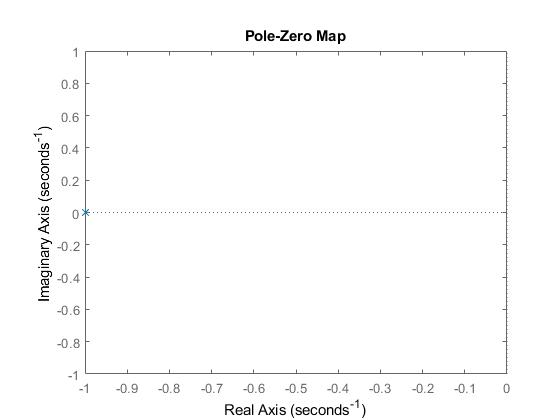
\includegraphics{Imagens/Lab2/tau1.jpg}

Como o polo da função de transferência se encontra na SPE, conclui-se que o sistema se compartará de uma forma estável.

\hypertarget{parte-2}{%
\paragraph*{Parte 2}\label{parte-2}}
\addcontentsline{toc}{paragraph}{Parte 2}

Para \(\tau = 0.5\), temos a função de transferência dada por
\[
G(S)= \frac {1}{0.5s+1}.
\]

O código implementado no \texttt{Matlab} foi o apresentado abaixo.

\begin{Shaded}
\begin{Highlighting}[]
\VariableTok{g} \OperatorTok{=} \VariableTok{tf}\NormalTok{([}\FloatTok{1}\NormalTok{]}\OperatorTok{,}\NormalTok{ [}\FloatTok{0.5} \FloatTok{1}\NormalTok{])}
\NormalTok{[}\VariableTok{p}\OperatorTok{,} \VariableTok{z}\NormalTok{] }\OperatorTok{=} \VariableTok{pzmap}\NormalTok{(}\VariableTok{g}\NormalTok{)}
\VariableTok{pzmap}\NormalTok{(}\VariableTok{g}\NormalTok{)}
\end{Highlighting}
\end{Shaded}

Tendo como resultados de polos e zeros:

\begin{verbatim}
p =

    -2


z =

  0×1 empty double column vector
\end{verbatim}

Ou seja, a função de transferência não apresenta zeros e tem seu polo em \(s = -2\). A sua posição no plano é apresentada na figura abaixo

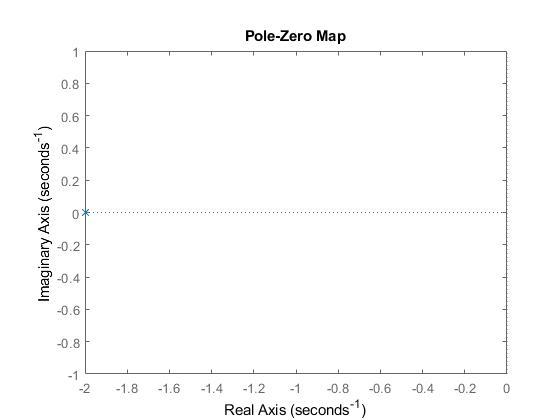
\includegraphics{Imagens/Lab2/tau2.jpg}

Como o polo da função de transferência se encontra na SPE, conclui-se que o sistema se compartará de uma forma estável. Também é possível concluir que o sistema alcanraça a estabilidade mais rápido para \(\tau = 0.5\).

\hypertarget{parte-3}{%
\paragraph*{Parte 3}\label{parte-3}}
\addcontentsline{toc}{paragraph}{Parte 3}

A simulação do sistema implementada em \texttt{Matlab} está apresentado na figura abaixo.

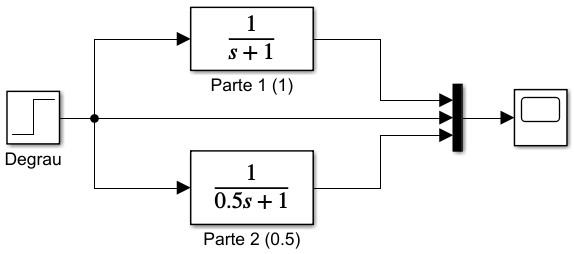
\includegraphics{Imagens/Lab2/sim1.jpg}

O resultado apresentado pelo \emph{scope} é apresentado na figura abaixo.

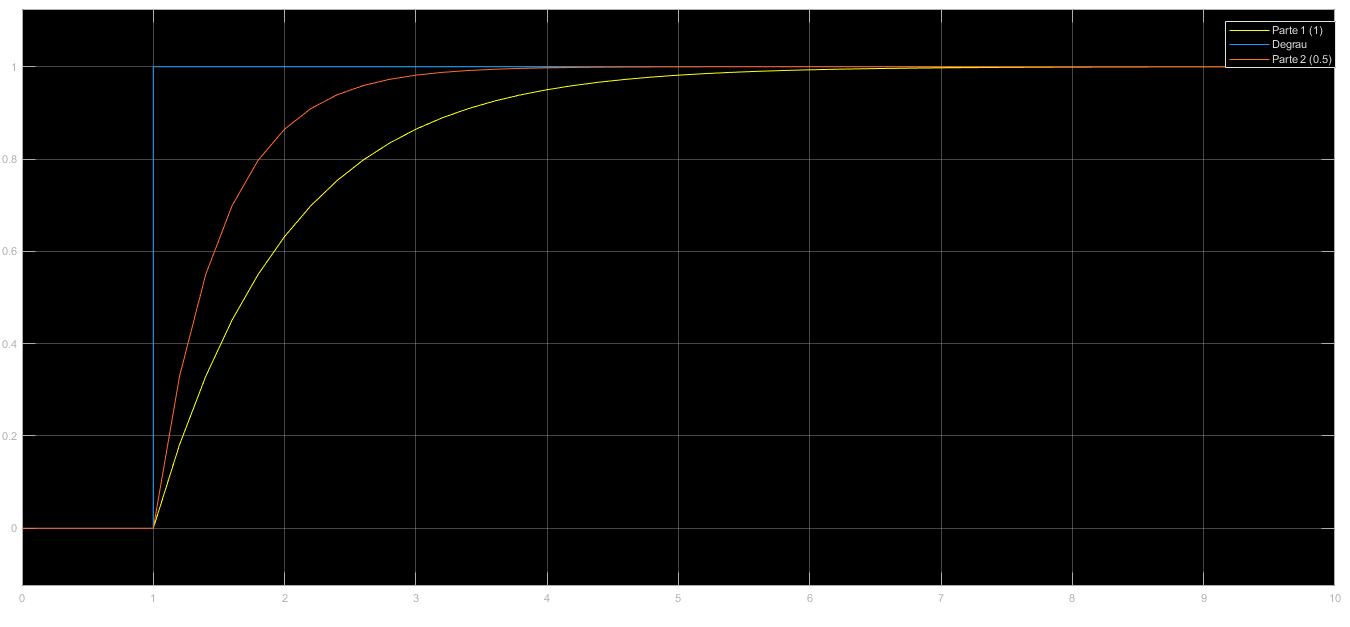
\includegraphics{Imagens/Lab2/resultSim1.jpg}

Percebe-se que, assim como esperado, o sistema se comporta de forma estável e tem uma convergência mais rápida para \(\tau = 0.5\).

\hypertarget{parte-4}{%
\paragraph*{Parte 4}\label{parte-4}}
\addcontentsline{toc}{paragraph}{Parte 4}

Para a última etapa temos a função de transferência dada por
\[
G(S)= \frac {1}{s-1}.
\]

O código implementado no \texttt{Matlab} foi o apresentado abaixo.

\begin{Shaded}
\begin{Highlighting}[]
\VariableTok{g} \OperatorTok{=} \VariableTok{tf}\NormalTok{([}\FloatTok{1}\NormalTok{]}\OperatorTok{,}\NormalTok{ [}\FloatTok{1} \OperatorTok{{-}}\FloatTok{1}\NormalTok{])}
\NormalTok{[}\VariableTok{p}\OperatorTok{,} \VariableTok{z}\NormalTok{] }\OperatorTok{=} \VariableTok{pzmap}\NormalTok{(}\VariableTok{g}\NormalTok{)}
\VariableTok{pzmap}\NormalTok{(}\VariableTok{g}\NormalTok{)}
\end{Highlighting}
\end{Shaded}

Tendo como resultados de polos e zeros:

\begin{verbatim}
p =

    1


z =

  0×1 empty double column vector
\end{verbatim}

Ou seja, a função de transferência não apresenta zeros e tem seu polo em \(s = 1\). A sua posição no plano é apresentada na figura abaixo

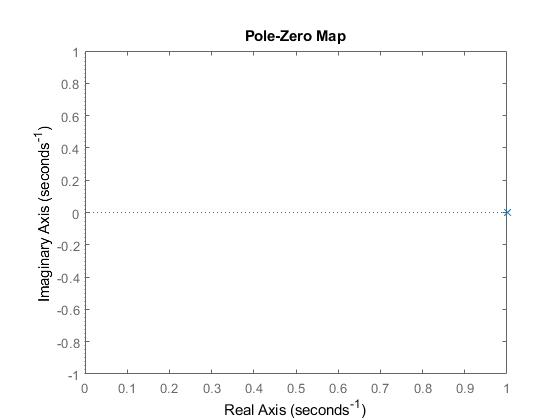
\includegraphics{Imagens/Lab2/tau3.jpg}

Como o polo da função de transferência se encontra na SPD, conclui-se que o sistema se compartará de uma forma instável. A simulação em \texttt{Matlab} está apresentada na figura abaixo.

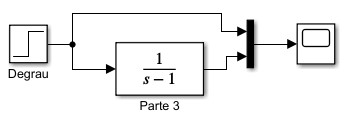
\includegraphics{Imagens/Lab2/sim2.jpg}

O resultado apresentado pelo \emph{scope} é apresentado na figura abaixo.

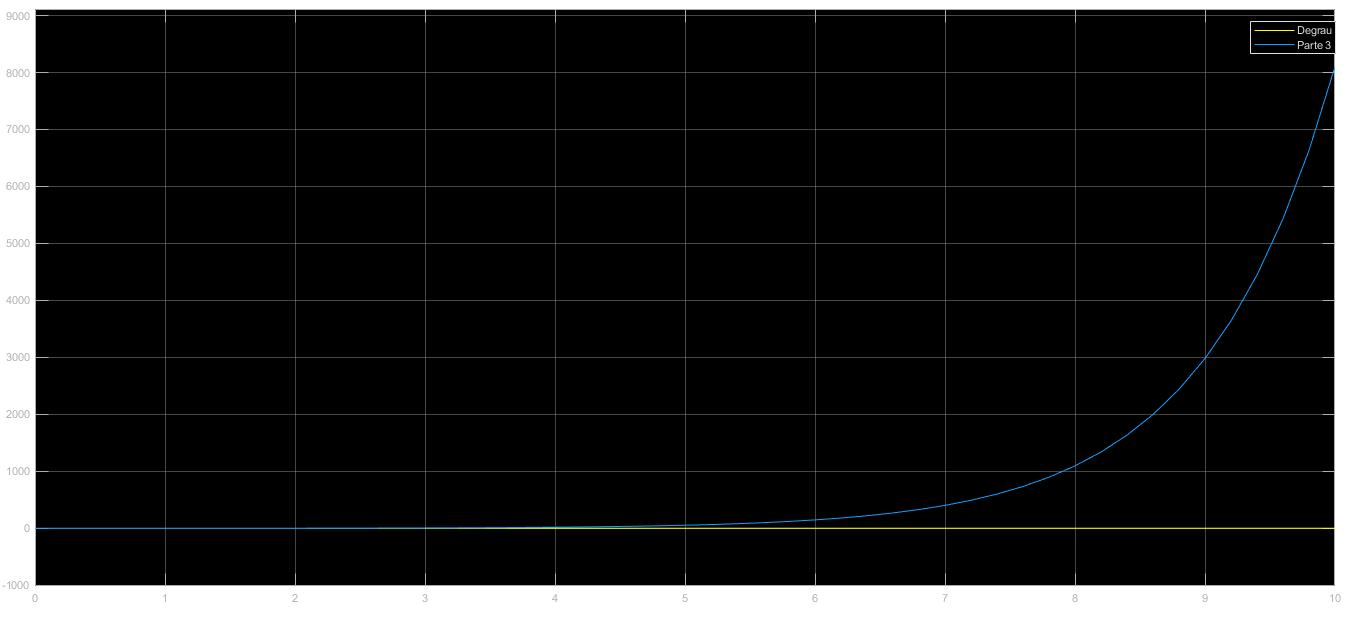
\includegraphics{Imagens/Lab2/resultSim2.jpg}

O resultado comprova o esperado. O sistema se comporta de forma instável para a função de transferência dada por \(G(s) = \frac {1}{s-1}\).

\hypertarget{problema-2}{%
\subsection*{Problema 2}\label{problema-2}}
\addcontentsline{toc}{subsection}{Problema 2}

Considere o sistema de primeira ordem (integrador)
\[
G(s) = \frac {1}{s}.
\]

Determine o pólo e a sua posição no plano \(s\) e simule para uma entrada do tipo degrau unitário e também para \(\sin {(t)}\) (para \(\sin {(t)}\), escolha \textbf{Max Step Size = 0.1} em \textbf{Simulation \(\implies\) Configurarion Parameters}). Note que a saída é a integral da entrada. Tais resultados eram esperados? Dica: relembre que \(Y(s) = G(s)U(s)\), e que se \(x(t) \iff X(S)\), então \(\int_0^t x(\tau) \mathrm{d}\tau \iff X(s)/s\).

\hypertarget{resoluuxe7uxe3o-1}{%
\subsubsection*{Resolução}\label{resoluuxe7uxe3o-1}}
\addcontentsline{toc}{subsubsection}{Resolução}

O código utilizado no \texttt{Matlab} é apresentado abaixo.

\begin{Shaded}
\begin{Highlighting}[]
\VariableTok{g} \OperatorTok{=} \VariableTok{tf}\NormalTok{([}\FloatTok{1}\NormalTok{]}\OperatorTok{,}\NormalTok{ [}\FloatTok{1} \FloatTok{0}\NormalTok{])}
\NormalTok{[}\VariableTok{p}\OperatorTok{,}\VariableTok{z}\NormalTok{] }\OperatorTok{=} \VariableTok{pzmap}\NormalTok{(}\VariableTok{g}\NormalTok{)}
\VariableTok{pzmap}\NormalTok{(}\VariableTok{g}\NormalTok{)}
\end{Highlighting}
\end{Shaded}

Obtendo como resultado:

\begin{verbatim}
p =

     0


z =

  0×1 empty double column vector
\end{verbatim}

Conclue-se então que a função de transferência \(G(s) = \frac {1}{s}\) não tem zeros e tem pólo em \(s = 0\). O mapa da posição no plano é mostrado na figura abaixo.

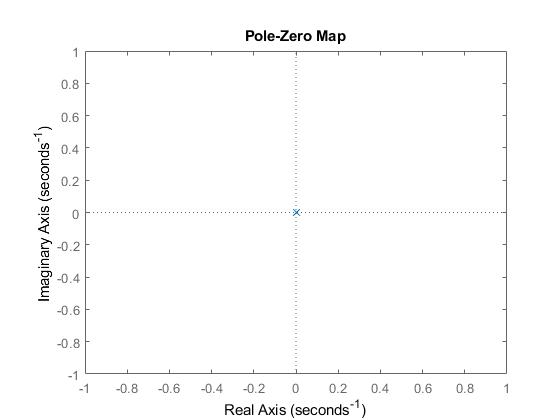
\includegraphics{Imagens/Lab2/prob2.jpg}

Isso mostra que o sistema é um caso crítico. Neste caso a resposta em regime permanente do sistema a uma entrada de amplitude limitada será uma senóide.

A simulação feita em \texttt{Matlab} está apresentada na figura abaixo.

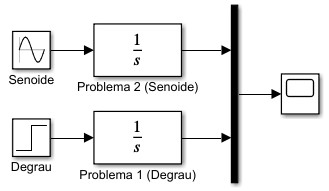
\includegraphics{Imagens/Lab2/simP2.jpg}

O resultado da simulação é apresentado na figura abaixo.

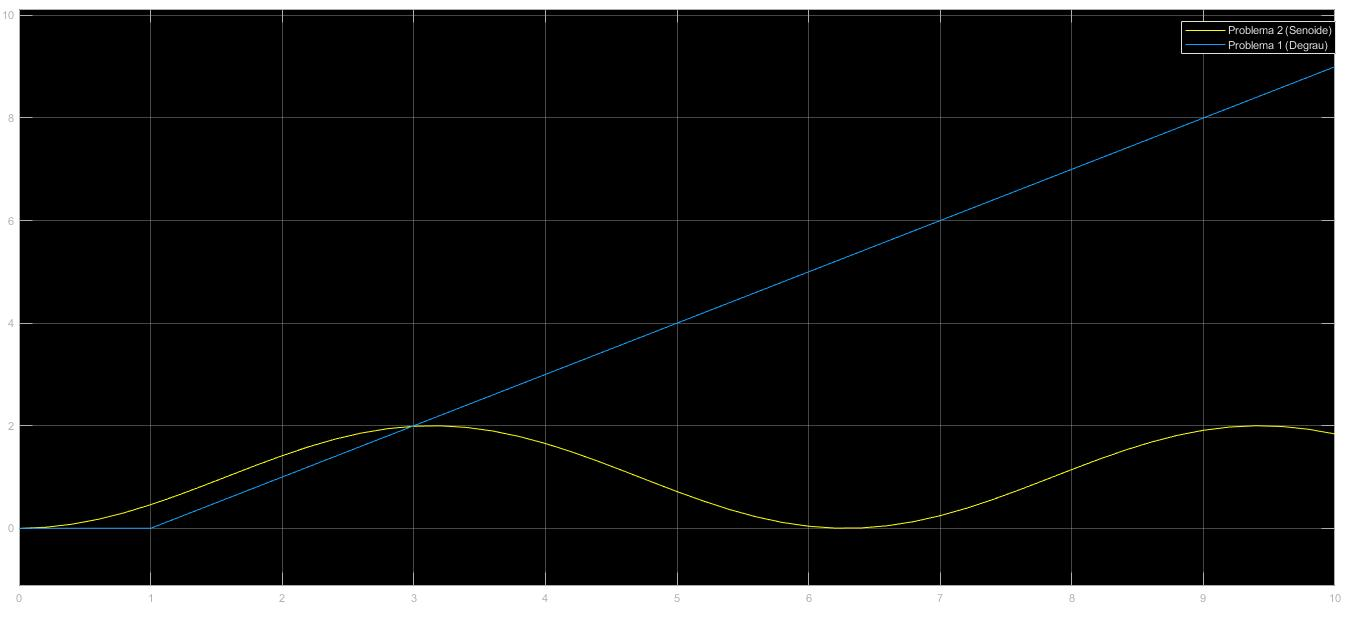
\includegraphics{Imagens/Lab2/prob2B.jpg}

O resultados eram esperados, uma vez que em um estado crítico a função de transferência pode estar em um estado permanente senoidal caso a entrada seja senoidal ou pode divergir caso a entrada seja um sinal constante.

\hypertarget{problema-3}{%
\subsection*{Problema 3}\label{problema-3}}
\addcontentsline{toc}{subsection}{Problema 3}

Considere o sistema de segunda ordem
\[
G(s) = \frac {1}{s^2 +25}.
\]

Determine os pólos e suas posições no plano \(s\). Simule para as seguintes entradas: degrau unitário, \(\sin (4t)\), \(\sin(6t)\). Observe que a saída é limitada. Agora, semule para a entrada \(\sin(5t)\). Note que a amplitude de saída cresce indefinidamente. Tal fenômeno é denominado de \emph{ressonância}. De moro mais geral, para
\[
G(s) = \frac {1}{s^2+\omega_0^2},
\]
teremos ressonância quando aplicamos uma entrada senoidal da forma \(\sin(\omega_0t + \phi)\). Note que a \emph{frequência de ressonância} \(\omega_0\) é igual a parte imaginária dos pólos de \(G(s)\).

\hypertarget{resoluuxe7uxe3o-2}{%
\subsubsection*{Resolução}\label{resoluuxe7uxe3o-2}}
\addcontentsline{toc}{subsubsection}{Resolução}

O código utilizado no \texttt{Matlab} é apresentado abaixo.

\begin{Shaded}
\begin{Highlighting}[]
\VariableTok{g} \OperatorTok{=} \VariableTok{tf}\NormalTok{([}\FloatTok{1}\NormalTok{]}\OperatorTok{,}\NormalTok{ [}\FloatTok{1} \FloatTok{0} \FloatTok{25}\NormalTok{])}
\NormalTok{[}\VariableTok{p}\OperatorTok{,}\VariableTok{z}\NormalTok{] }\OperatorTok{=} \VariableTok{pzmap}\NormalTok{(}\VariableTok{g}\NormalTok{)}
\VariableTok{pzmap}\NormalTok{(}\VariableTok{g}\NormalTok{)}
\end{Highlighting}
\end{Shaded}

Obtendo como resultado:

\begin{verbatim}
p =

   0.0000 + 5.0000i
   0.0000 - 5.0000i


z =

  0×1 empty double column vector
\end{verbatim}

Conclue-se então que a função de transferência \(G(s) = \frac {1}{s^2 +25}\) não tem zeros e tem pólo em \(s = \pm 5i\). O mapa da posição no plano é mostrado na figura abaixo.

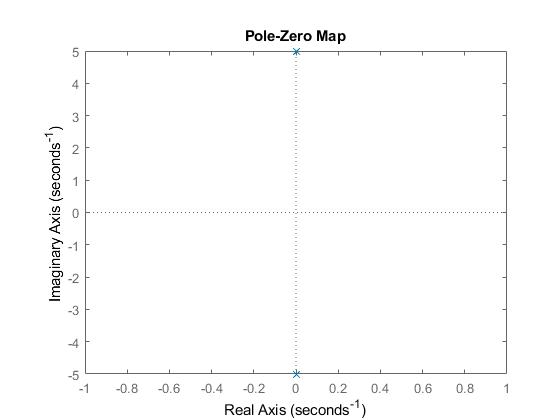
\includegraphics{Imagens/Lab2/prob3.jpg}

De acordo com o mapa de posição, pode-se concluir que a função de transferência é classificada como um caso crítico. A figura abaixo apresenta o modelo de simulação criado no \texttt{Simulink}.

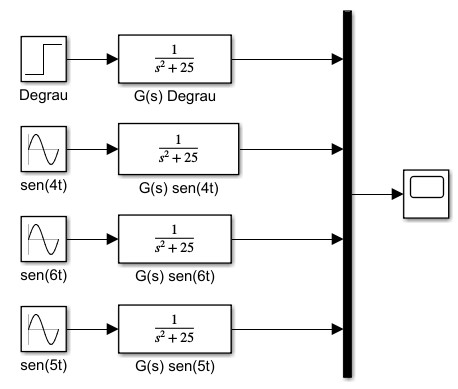
\includegraphics{Imagens/Lab2/modelSim3.jpg}

O resultado da simulação é apresentado abaixo.

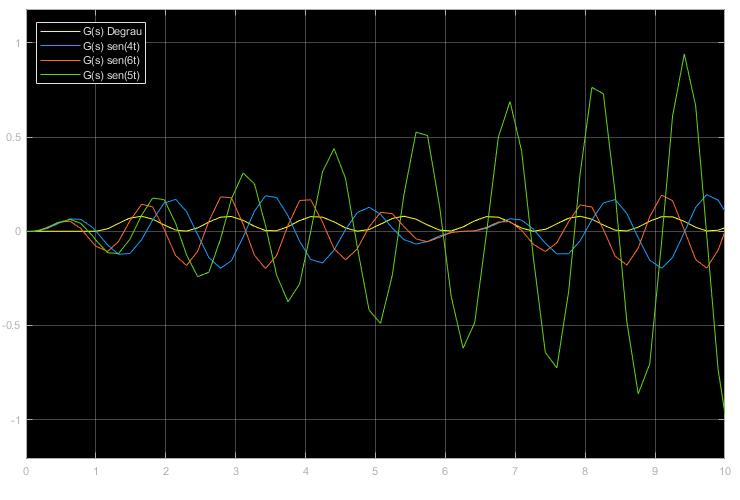
\includegraphics{Imagens/Lab2/prob3Sim.jpg}

É fácil perceber que o modelo se comporta de maneira instável com a entrada \(u(t) = \sin(5t)\), se mostrando estável nas demais situações.

\hypertarget{problema-4}{%
\subsection*{Problema 4}\label{problema-4}}
\addcontentsline{toc}{subsection}{Problema 4}

Considere o sistema de segunda orde
\[
G(s) = \frac {1.6}{(s+1)(s+2)} = \frac {0.8}{0.5s^2+1.5s+1}.
\]

Determine os pólos e suas posições no plano \(s\) e simule para uma entrada do tipo degrau unitário. Note que não há sobressinal. Tal resultado era esperado? Justifique.

Agora, adicionando um zero, temos
\[
G(s) = \frac {1.6(\beta s+1)}{(s+1)(s+2)} = \frac {0.8(\beta s+1)}{0.5s^2 +1.5s +1},
\]
onde \(\beta = 0.1\), \(\beta = 0.6\), \(\beta = 0.99\), \(\beta = 1.2\), \(\beta = 2\), \(\beta = 10\). Para cada valor de \(\beta\), determine os pólos e zeros, suas posições no plano \(s\) e simule para uma entrada do tipo degrau unitário. Analise e compare os resultados. Note que dependendo da posição do zero o sobressinal será maior ou menor, podendo também não estar presente.

\hypertarget{resoluuxe7uxe3o-3}{%
\subsubsection*{Resolução}\label{resoluuxe7uxe3o-3}}
\addcontentsline{toc}{subsubsection}{Resolução}

Utilizando a função \texttt{pzmap()} do \texttt{Matlab} para encontrar os pólos da função de transferência \(G(s) = \frac {0.8}{0.5s^2+1.5s+1}\) temos que a função não possui zeros e possui polos para \(s = -2\) e \(s = -1\). O mapa de posições é apresentado na figura abaixo.

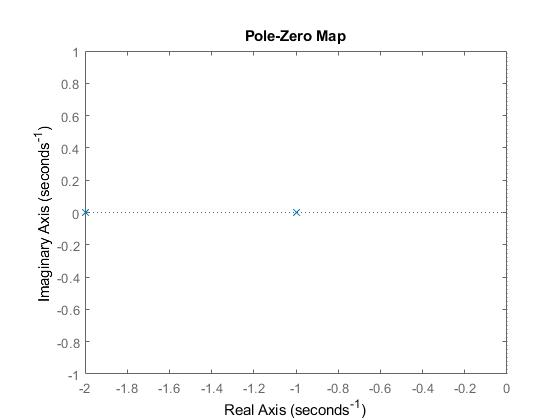
\includegraphics{Imagens/Lab2/prob4.jpg}

O resultado da função de transferência é apresentado na figura abaixo.

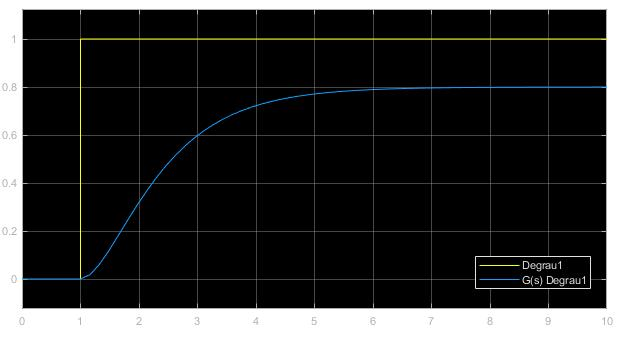
\includegraphics{imagens/Lab2/prob41.jpg}

Agora, considerando a função de transferência
\[
G(s) = \frac {0.8(\beta s+1)}{0.5s^2+1.5s+1},
\]
e substituindo os valores de \(\beta\) pelos valores propostos temos os valores de zero e pólo apresentados na tabela abaixo.

\begin{table}

\caption{\label{tab:unnamed-chunk-6}Valores de Pólo e Zero variando $\beta$}
\centering
\begin{tabular}[t]{lll}
\toprule
  & Pólos & Zeros\\
\midrule
$\beta = 0.1$ & {-2, -1} & -10.0\\
$\beta = 0.6$ & {-2, -1} & -1.67\\
$\beta = 0.99$ & {-2, -1} & -1.01\\
$\beta = 1.2$ & {-2, -1} & -0.83\\
$\beta = 2$ & {-2, -1} & -0.50\\
\addlinespace
$\beta = 10$ & {-2, -1} & -0.10\\
\bottomrule
\end{tabular}
\end{table}

Os gráficos de posição estão apresentados abaixo.

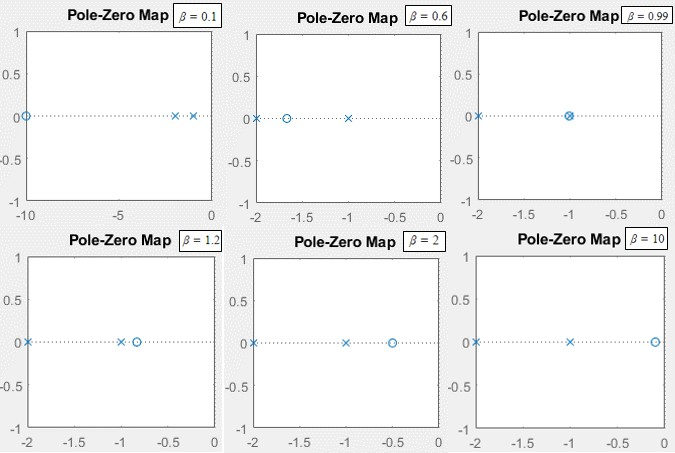
\includegraphics{Imagens/Lab2/prob4Varios.jpg}

A simulação feita em \texttt{Matlab} está apresentada na figura abaixo.

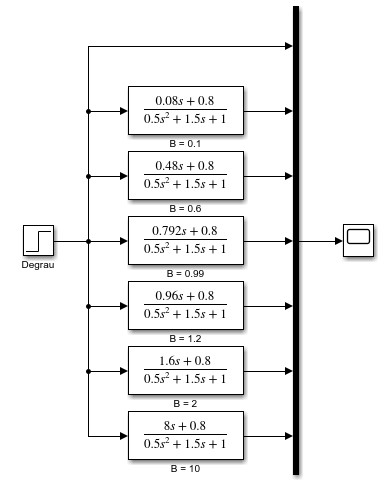
\includegraphics{Imagens/Lab2/modelSim4.jpg}

O resultado da simulação está apresentado na figura abaixo.

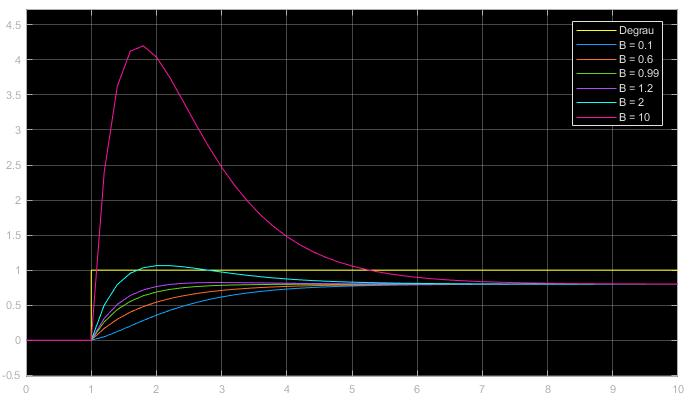
\includegraphics{Imagens/Lab2/prob4SimResult.jpg}

É possível perceber que quanto mais alto o valor de \(\beta\) maior o sobressinal. Também é possível perceber que há um intervalo no qual o tempo de reação aumenta, encontrando seu tempo de reação mínimo, voltando então a aumentar.

\hypertarget{problema-5}{%
\subsection*{Problema 5}\label{problema-5}}
\addcontentsline{toc}{subsection}{Problema 5}

Considere o sistema de segunda ordem
\[
G(s) = \frac {0.9}{s^2+s+1}.
\]

Determine os pólos e suas posições no plano \(s\) e simule para uma entrada do tipo degrau unitário. Note que há sobressinal. Tal resultado era esperado? Justifique.

Agora, adicionando um zero, temos
\[
G_z(s) = \frac {0.9(\beta s+1)}{s^2+s+1},
\]
onde \(\beta = 0.05\), \(\beta = 0.5\), \(\beta = 1\) e \(\beta = 2.5\). Para cada valor de \(\beta\) determine os pólos e zeros, suas posições no plano \(s\) e simule para uma entrada do tipo degrau unitário. Analise e compare os resultados.

\hypertarget{resoluuxe7uxe3o-4}{%
\subsubsection*{Resolução}\label{resoluuxe7uxe3o-4}}
\addcontentsline{toc}{subsubsection}{Resolução}

Utilizando a função \texttt{pzmap()} do \texttt{Matlab} para encontrar os pólos da função de transferência \(G(s) = \frac {0.9}{s^2+s+1}\) temos que a função não possui zeros e possui polos para \(s = -0.5 + 0.86i\) e \(s = -0.5 -0.86i\). O mapa de posições é apresentado na figura abaixo.

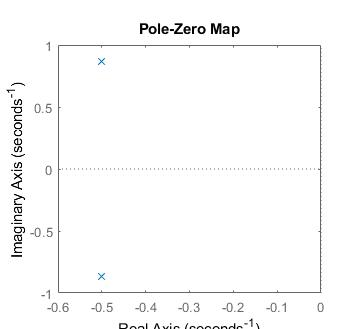
\includegraphics{Imagens/Lab2/prob5.jpg}

O resultado da função de transferência é apresentado na figura abaixo.

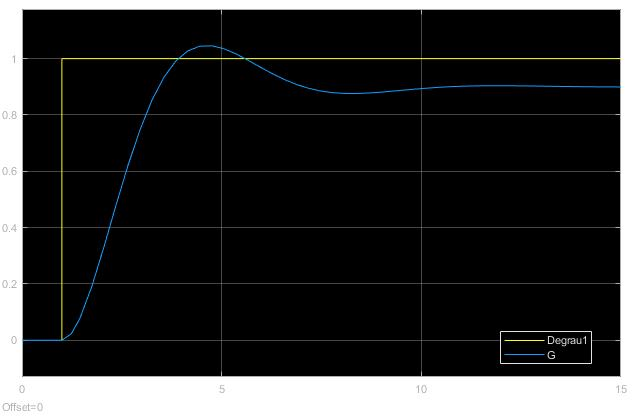
\includegraphics{imagens/Lab2/prob5Sim.jpg}

É possível perceber que há sobressinal.

Agora, considerando a função de transferência \(G_z(s) = \frac {0.9(\beta s+1)}{s^2+s+1}\), e substituindo os valores de \(\beta\) pelos valores propostos temos os valores de zero e pólo apresentados na tabela abaixo.

\begin{table}

\caption{\label{tab:unnamed-chunk-7}Valores de Pólo e Zero variando $\beta$}
\centering
\begin{tabular}[t]{lll}
\toprule
  & Pólos & Zeros\\
\midrule
$\beta = 0.05$ & {$-0.5 \pm 0.86i$} & -20.0\\
$\beta = 0.5$ & {$-0.5 \pm 0.86i$} & -2.0\\
$\beta = 1$ & {$-0.5 \pm 0.86i$} & -1.0\\
$\beta = 2.5$ & {$-0.5 \pm 0.86i$} & -0.4\\
\bottomrule
\end{tabular}
\end{table}

Os gráficos de posição estão apresentados abaixo.

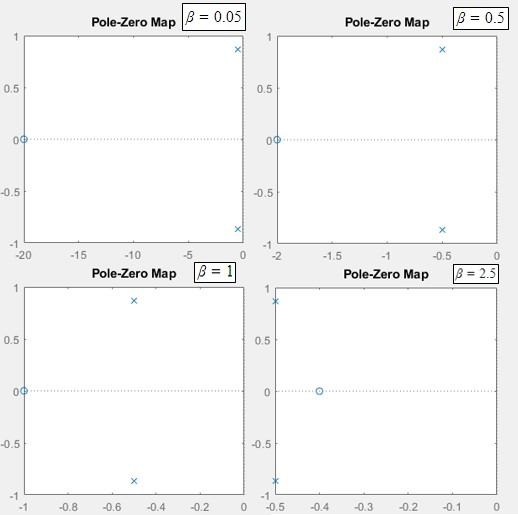
\includegraphics{Imagens/Lab2/prob5Varios.jpg}

A simulação feita em \texttt{Matlab} está apresentada na figura abaixo.

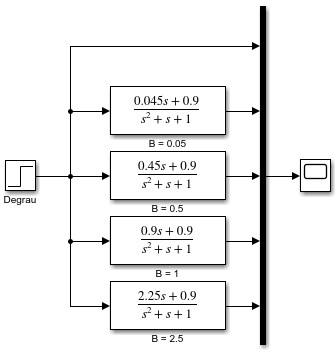
\includegraphics{Imagens/Lab2/modelSim5.jpg}

O resultado da simulação está apresentado na figura abaixo.

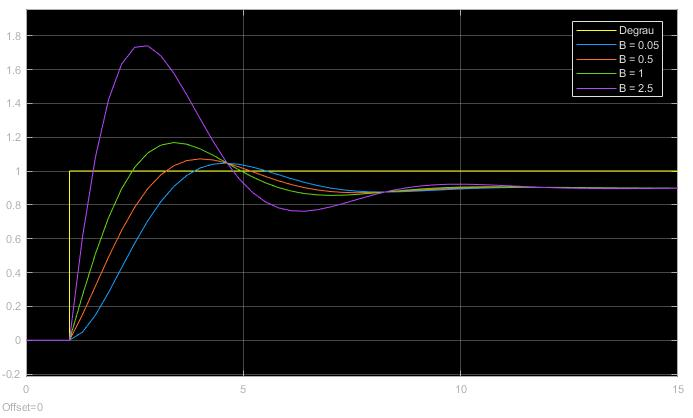
\includegraphics{Imagens/Lab2/prob5SimResult.jpg}

É possível perceber que quanto mais alto o valor de \(\beta\) maior o sobressinal e o tempo de resposta do sistema.

\hypertarget{problema-6}{%
\subsection*{Problema 6}\label{problema-6}}
\addcontentsline{toc}{subsection}{Problema 6}

Considere o sistema de segunda ordem de fase não-mínima
\[
G(s) = \frac {-s+1}{0.5s^2+1.5s+1}.
\]

Determine os pólos e o zero, suas posições no plano \(s\) e simule para uma entrada do tipo degrau unitário. Note que a resposta é negativa nos instantes iniciais. Justificaremos tal comportamento no que se segue.

Escrevemos
\[
G(s) = \frac {-s+1}{0.5s^2+1.5s+1} = \overbrace{\frac {1}{0.5s^2+1.5s+1}}^{G_1(s)} - \overbrace{\frac {s}{0.5s^2+1.5s+1}}^{G_2(s) = sG_1(S)}.
\]

Assim,
\[
Y(s) = G(s)U(s) = G_1(s)U(s)-G_2(s)U(s) = \underbrace{G_1(s)U(s)}_{Y_1(s)} - \underbrace{sG_1(s)U(s)}_{Y_2(s) = sY_1(s)}.
\]

Relembre-se que se \(x(t) \iff X(S)\) com \(x(0) = 0\), então \(dx(t)/dt \iff sX(s)\). Portanto,
\[
y(t) = y_1(t)-y_2(t)=y_1(t)- \frac {dy_1(t)}{dt}.
\]

Verifique a validade da equação acima no Simulink (utilize o bloco \textbf{Derivative} no Simulink) para uma entrada do tipo degrau unitário. Analise o motivo da resposta ser negativa nos instantes iniciais.

\hypertarget{resoluuxe7uxe3o-5}{%
\subsubsection*{Resolução}\label{resoluuxe7uxe3o-5}}
\addcontentsline{toc}{subsubsection}{Resolução}

\begin{align}
    r  = \frac{1}{n-1} \sum_{i=1}^{n} \frac{(X_i - \bar{X})(Y_i - \bar{Y})}{S_xS_y}
\end{align}

\hypertarget{identificauxe7uxe3o-de-sistemas}{%
\chapter{Identificação de Sistemas}\label{identificauxe7uxe3o-de-sistemas}}

\hypertarget{apresentauxe7uxe3o-do-laboratuxf3rio-1}{%
\section{Apresentação do Laboratório}\label{apresentauxe7uxe3o-do-laboratuxf3rio-1}}

\hypertarget{objetivo-1}{%
\subsection{Objetivo}\label{objetivo-1}}

Nesta experiência, veremos como modelar matematicamente um sistema linear por uma Função de Transferência. Identificaremos os parâmetros de uma Função de Transferência de primeira e de segunda ordem. Compararemos a dinâmica do sistema com a do modelo matemático.

\hypertarget{modelagem-de-sistemas-lineares}{%
\subsection{Modelagem de Sistemas Lineares}\label{modelagem-de-sistemas-lineares}}

Encontrar um modelo matemático que capture as características dinâmicas relevantes de um sistema real é de fundamental importância para a análise e controle do sistema. No Laboratório 1 estudamos um modelo linear com motor CC. Tal modelo pode ser obtido a partir das leis da física (mecânica e eletromagnetismo) e os valores dos parâmetros dependem de constantes e coeficientes físicos (indutância do enrolamento, resistência do enrolamento, constante de torque do motor, coeficiente de atrito ciscoso). Em situações reais, não conheceremos uma estimativa para os mesmos. Por exemplo, todo resistor possui um valor normal e uma faixa de tolerância percentual (e.g.~\(R = 100 \Omega \pm 5\%\)). Além disso, muitas vezes a determinação de um modelo matemático para um sistema a partir de leis naturais é extremamente difícil e, mesmo no caso em que isso é possível, o modelo obtido pode ser demasiadamente complexo para ser estudado matematicamente.

Devido às dificuldades que acabamos de expor, em geral buscamos um modelo matemático relativamente simples mas que capture, ao menos aproximadamente, as características dinâmicas relevantes do sistema. Assim, primeiramente fixamos um modelo (\emph{modelagem} do sistema) e em seguida determinamos de maneira aproximada o valor de seus parâmetros (\emph{identificação} dos parâmetros).

Nesta experiência, consideraremos apenas sistemas lineares que possam ser modelados por uma função de Transferência \(G(s)\) de primeira ordem ou de segunda ordem. Veremos então como identificar os parâmetros de \(G(s)\).

\hypertarget{identificauxe7uxe3o-de-sistemas-de-primeira-ordem}{%
\subsection{Identificação de sistemas de primeira ordem}\label{identificauxe7uxe3o-de-sistemas-de-primeira-ordem}}

Toda Função de Transferência \(G(s)\) de primeira ordem pode ser escrita na forma padrão como

\begin{align}
G(s) = \frac{K}{\tau s+1}. \label{eq:eq1}
\end{align}

Supunha que \(G(s)\) é estável, ou seja, \(\tau > 0\). considere uma entrada \(u(t) = A\) do tipo degrau de magnitude \(A\). Temos que a saída correspondente é
\[
y(t) = AK(1- e^{\frac {-t}{\tau}}).
\]

O valor da saída em regime permanente é
\[
y(\infty) = AK,
\]
e o tempo de acomodação de \(5\%\) é dado por
\[
0.95KA = KA(1- e^{\frac {-t_s(5\%)}{\tau}}) \implies t_s(5\%) =3 \tau.
\]

Isto é ilustrado na figura 1.

\begin{figure}
\centering
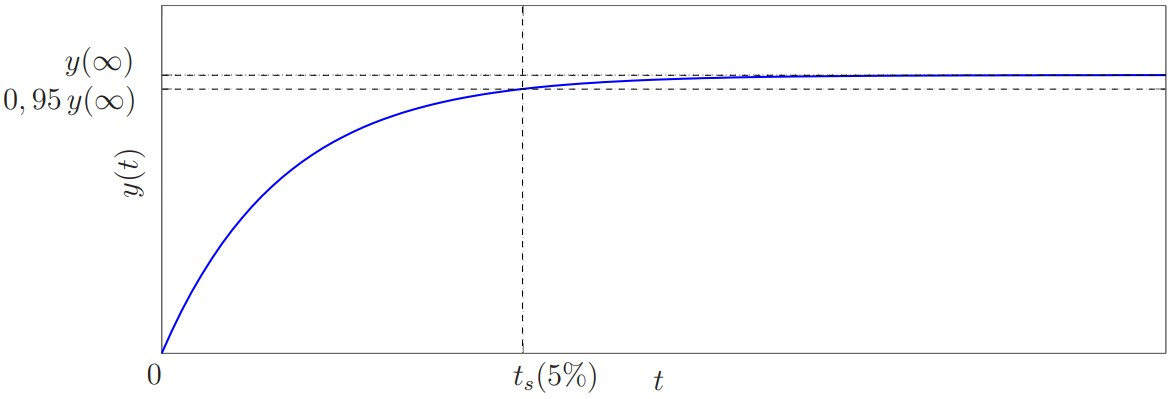
\includegraphics{Imagens/Lab3/Explicação/fig1.jpg}
\caption{Figura 1: Resposta de um sistema de primeira ordem ao degrau.}
\end{figure}

Logo,

\begin{align}
K = \frac{y(\infty)}{A},  \tau = \frac {t_s(5\%)}{3}. \label{eq:eq2}
\end{align}

\hypertarget{identificauxe7uxe3o-de-sistemas-de-segunda-ordem}{%
\subsection{Identificação de Sistemas de Segunda Ordem}\label{identificauxe7uxe3o-de-sistemas-de-segunda-ordem}}

Toda Função de Transferência \(G(s)\) de segunda ordem com pólos não-nulos pode ser escrita como

\begin{align}
G(s) = \frac {K \omega_n^2}{s^2+2\xi \omega_n+ \omega_n^2}, \label{eq:eq3}
\end{align}

onde \(\omega_n > 0\). Os pólos de \(G(s)\) são:
\[
p_{1,2} = - \xi \omega_n \pm \sqrt{\xi^2 -1}.
\]

Temos as seguintes situações:

\begin{enumerate}
\def\labelenumi{\arabic{enumi}.}
\tightlist
\item
  Sistema não-amortecido (\(\xi = 0\)): os pólos são complexos com \(p_{1,2} = \pm j \omega_n\), e a resposta a uma entrada do tipo degrau é senoidal.
\item
  Sistema sub-amortecido (\(0< \xi <1\)): os pólos são complexos com \(p_{1,2} = - \xi \omega_n \pm j \omega_n\sqrt{1 - \xi^2}\) e a resposta ao degrau apresenta oscilação e sobressinal.
\item
  Sistema criticamente amortecido (\(\xi = 1\)): os pólos são reais e iguais com \(p_{1,2} = -\xi \omega_n\) e a resposta ao degrau não apresenta oscilação nem sobressinal.
\item
  Sistema super-amortecido (\(\xi >1\)): os pólos são reais, negativos e diferentes e a resposta ao degrau não apresenta oscilação nem sobressinal.
\item
  Sistema instável (\(\xi < 0\)): os pólos possuem parte real positiva.
\end{enumerate}

\hypertarget{sistemas-sub-amortecidos}{%
\subsubsection{Sistemas sub-amortecidos}\label{sistemas-sub-amortecidos}}

Suponha que \(G(s)\) é estável com \(0 < \xi < 1\) (sub-amortecido). Considere uma entrada \(u(t) = A\) do tipo degrau de magnitude \(A\). A resposta correspondente \(y(t)\) é ilustrada na figura 2.

\begin{figure}
\centering
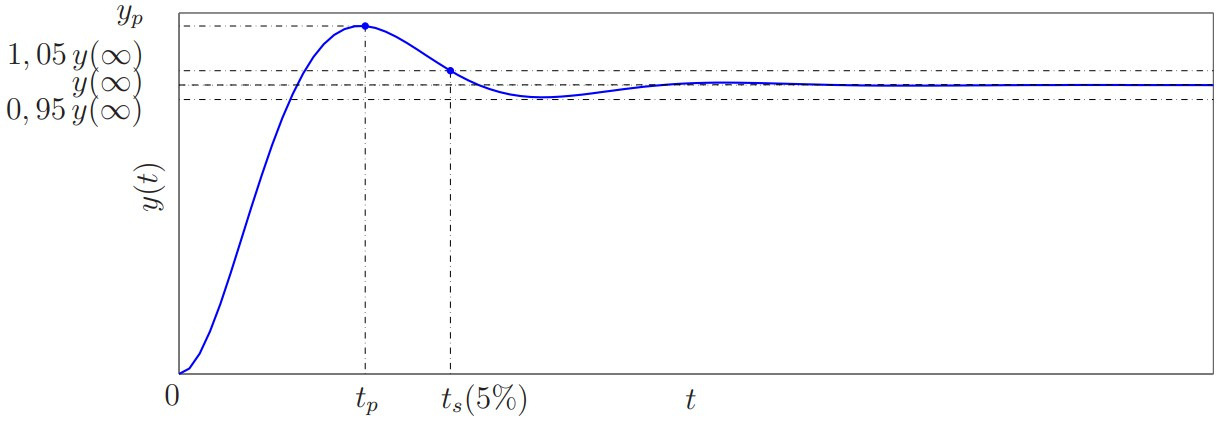
\includegraphics{Imagens/Lab3/Explicação/fig2.jpg}
\caption{Figura 2: Resposta de um sistema de segunda ordem sub-amortecido ao degrau.}
\end{figure}

Temos que
\[
y(\infty) = KA, \quad M_p= \frac {y_p-y(\infty)}{y(\infty)} = e^{\frac {-(\xi \pi)}{\sqrt{1-\xi^2}}}, \quad
t_p = \frac {\pi}{\omega_n\sqrt{1-\xi^2}}.
\]

Logo,

\begin{align}
K = \frac {y(\infty)}{A}, \quad M_p = \frac {y_p - y(\infty)}{y(\infty)}, \quad \xi = \sqrt{\frac {(\ln{M_p})^2}{(\ln{M_p})^2+\pi^2}}, \quad \omega_n = \frac {\pi}{t_p\sqrt{1-\xi^2}}.  \label{eq:eq4}
\end{align}

\hypertarget{sistemas-criticamente-amortecidos-e-super-amortecidos}{%
\subsubsection{Sistemas criticamente amortecidos e super-amortecidos}\label{sistemas-criticamente-amortecidos-e-super-amortecidos}}

Suponha que \(G(s)\) é estável com \(\xi \geq 1\) (criticamente amortecido ou super-amortecido). Neste caso, os dois pólos de \(G(s)\) são reais e a resposta ao degrau se assemelha ao de um sistema de primeira ordem (não apresenta oscilação nem sobressinal). Podemos identificar \(G(s)\) indiretamente através da identificação da Função de Transferência \(F(s)\) em malha-fechada. Considere o diagrama de blocos em malha-fechada mostrando na Figura 3, onde \(K_c > 0\) é o ganho de um controlador proporcional e \(r\) é a referência.

\begin{figure}
\centering
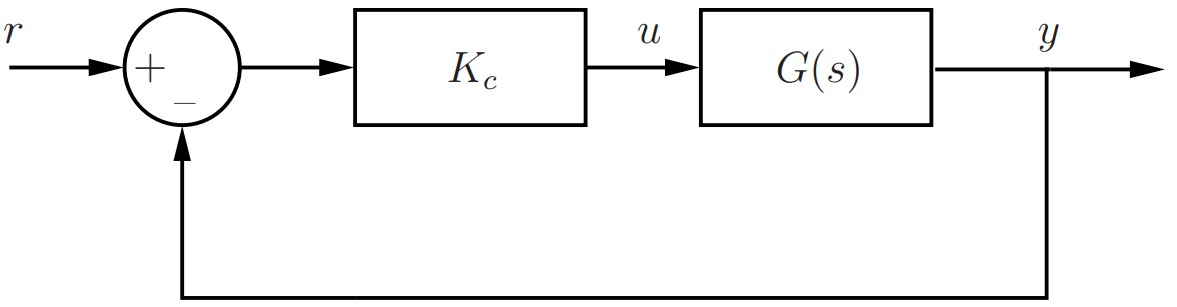
\includegraphics{Imagens/Lab3/Explicação/fig3.jpg}
\caption{Figura 3: Diagrama de blocos em malha-fechada.}
\end{figure}

Relembre que
\[
F(s) = \frac {Y(s)}{R(s)} = \frac {K_cG(s)}{1+K_cG(s)}.
\]

Para qualquer \(K_c > 0\), temos que \(F(s)\) é um sistema de segunda ordem estável. E, quando \(K_c > 0\) for suficientemente grade, temos que \(F(s)\) será um sistema de segunda ordem sub-amortecido. Assim, escolhemos \(K_c\) de modo que \(F(s)\) seja sub-amortecido e então identificamos \(F(s)\) conforme descrito na seção anterior aplicando uma referência \(r(t) = A\) do tipo degrau de magnitude \(A\). Desta maneira, identificaremos \(G(s)\) indiretamente pois

\begin{align}
F(s) = \frac {K_cG(s)}{1+K_cG(s)} \implies G(s) = \frac {F(s)}{K_c - K_cF(s)}.  \label{eq:eq5}
\end{align}

\hypertarget{procedimentos-1}{%
\section{Procedimentos}\label{procedimentos-1}}

\hypertarget{problema-1-1}{%
\subsection*{Problema 1}\label{problema-1-1}}
\addcontentsline{toc}{subsection}{Problema 1}

Aplique um degrau \(u(t) = 2\) no Sistema 1 do arquivo \texttt{MatLab3.mdl} do Simulink. Pelas características da resposta, modele o Sistema 1 como uma Função de Transferência \(G_1(s)%
\) de primeira ou segunda ordem. Em seguida, identifique os parâmetros do modelo utilizando a equação 3.2 ou 3.4. Compare a resposta do modelo identificado com a do Sistema 1.

\hypertarget{resoluuxe7uxe3o-6}{%
\subsubsection*{Resolução}\label{resoluuxe7uxe3o-6}}
\addcontentsline{toc}{subsubsection}{Resolução}

Simulando o sistema do modelo 1 obtemos o resultado abaixo.

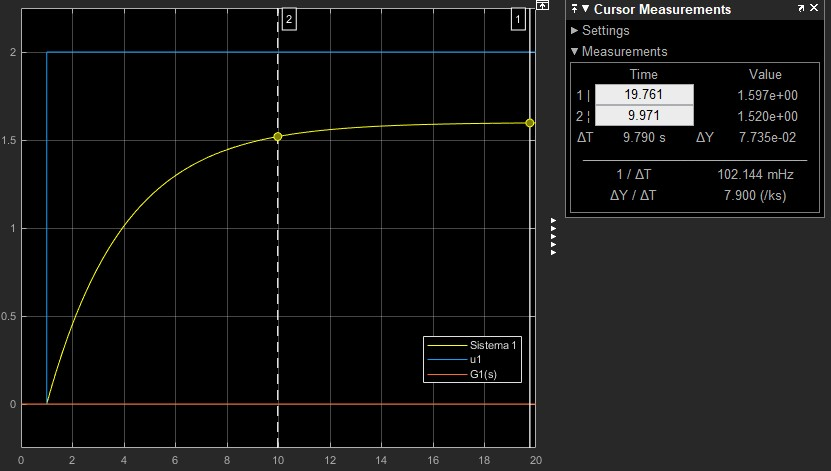
\includegraphics{Imagens/Lab3/Resolução/prob1A.jpg}

Pela curva feita espera-se que a Função de Transferência seja de primeira ordem. Utilizando as ferramentas fornecidas pelo \texttt{Simulink} foi estimado que
\[
y(\infty) = 1.6 \\
0.95y(\infty) = 1.52 \implies  t_s(5\%) = 9.97s \implies \tau = 3.33
\]

Assim,
\[
G_1(s) = \frac {0.8}{3.33s+1}.
\]

Simulando \(G_1(s)\), temos o resultado apresentado abaixo.

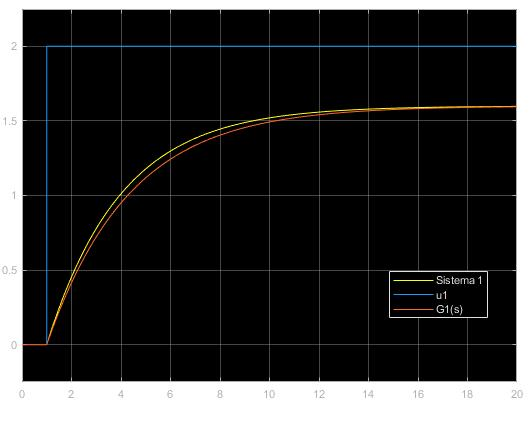
\includegraphics{Imagens/Lab3/Resolução/prob1B.jpg}

Percebe-se, assim, que a Função de Transferência \(G_1(s)\) se aproxima satisfatoriamente bem do Sistema 1.

\hypertarget{problema-2-1}{%
\subsection*{Problema 2}\label{problema-2-1}}
\addcontentsline{toc}{subsection}{Problema 2}

Aplique um degrau \(u(t) = 4\) no Sistema 2. Pelas características da resposta modele o Sistema 2 como uma Função de Transferência \(G_2(s)\) de primeira ou segunda ordem. Em seguida, identifique os parâmetros do modelo utilizando a equação 3.2 ou 3.4. Realize os cálculos na linha de comando do \texttt{Matlab} (\(\ln{(x)} \implies \log{(x)}\) e \(\sqrt{x} \implies \text{sqrt(x)}\)).Compare a resposta do modelo identificando com a do Sistema 2.

\hypertarget{resoluuxe7uxe3o-7}{%
\subsubsection*{Resolução}\label{resoluuxe7uxe3o-7}}
\addcontentsline{toc}{subsubsection}{Resolução}

Simulando o sistema do modelo 1 obtemos o resultado abaixo.

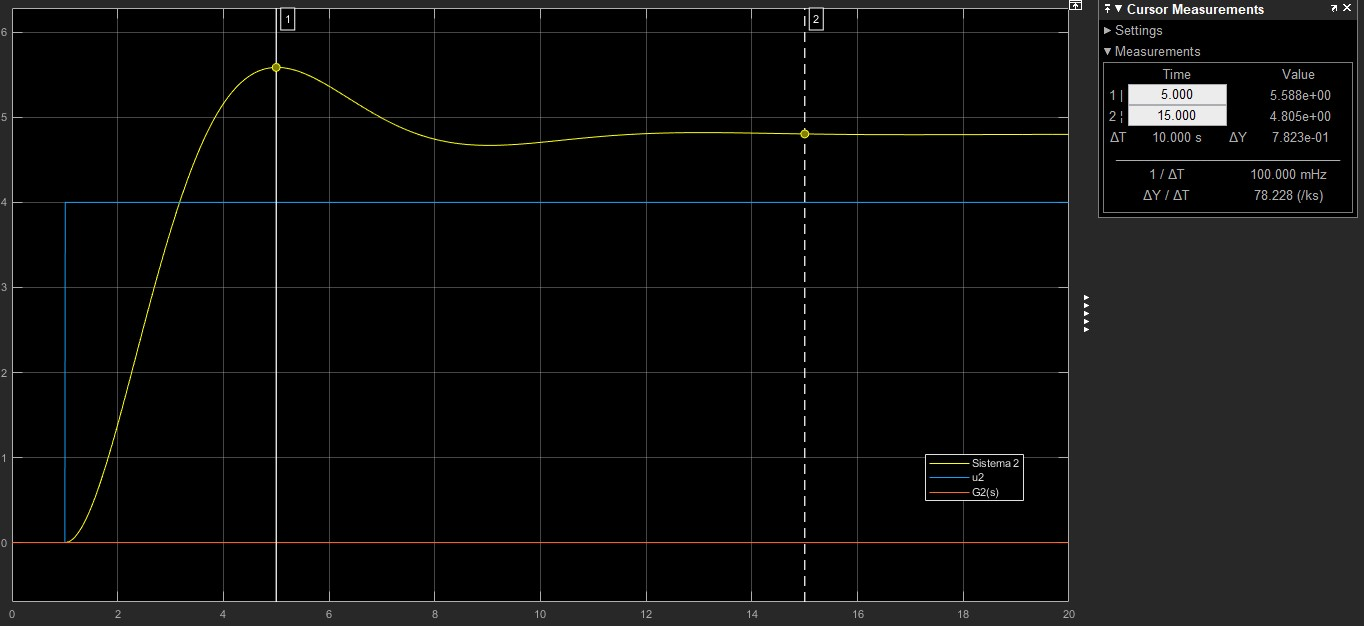
\includegraphics{Imagens/Lab3/Resolução/prob2A.jpg}

Pela curva feita espera-se que a Função de Transferência seja de segunda ordem. Utilizando as ferramentas fornecidas pelo \texttt{Simulink} foi estimado que
\[
y_p = 5.588\\
y(\infty) = 4.805 \\
t_p = 5s
\]

Dessa forma, aplicando as equações 3.4, temos que
\[
K = 1.2, \quad M_p = 0.163, \quad \xi = 0.5 \quad \text{e} \quad \omega_n = 0.7255.
\]

Dessa forma, a Função de Transferência \(G_2(s)\) será
\[
G_2(s) = \frac {0.6316}{s^2 + 0.7255s + 0.5264}.
\]
Simulando \(G_2(s)\), temos o resultado apresentado abaixo.

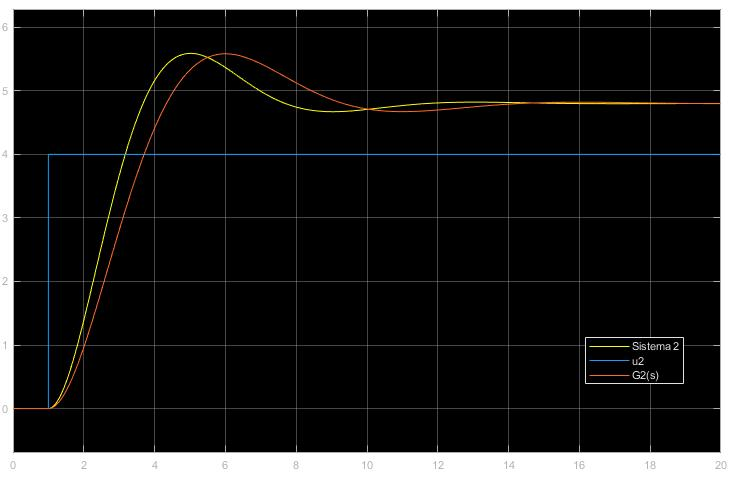
\includegraphics{Imagens/Lab3/Resolução/prob2B.jpg}

Percebe-se, assim, que a Função de Transferência \(G_2(s)\) se assemelha ao Sistema 2,porém, com menor precisão que a função \(G_1(s)\) se aproximou do Sistema 2.

\hypertarget{problema-3-1}{%
\subsection*{Problema 3}\label{problema-3-1}}
\addcontentsline{toc}{subsection}{Problema 3}

\hypertarget{parte-a}{%
\subsubsection*{Parte A}\label{parte-a}}
\addcontentsline{toc}{subsubsection}{Parte A}

Aplique um degrau \(u(t) = 3\) no Sistema 3. Obtenha um modelo aproximado para o Sistema 3 como uma Função de Transferência \(G(s)\) de primeira ordem. Agora implemente o diagrama de blocos em malha fechada da Figura 3 para o Sistema 3 com \(r(t) = 1\) do tipo degrau e \(K_c = 3\)Observamos que, na Figura 3, se \(G(s)\) é de primeira ordem, então a Função de Transferência em malha fechada \(F(s)\) também será de primeira ordem para qualquer valor de \(K_c > 0\). A resposta do Sistema 3 em malha-fechada está de acordo com tal propriedade? O que pode estar errado?

\hypertarget{resoluuxe7uxe3o-8}{%
\paragraph*{Resolução}\label{resoluuxe7uxe3o-8}}
\addcontentsline{toc}{paragraph}{Resolução}

Simulando o sistema do modelo 1 obtemos o resultado abaixo.

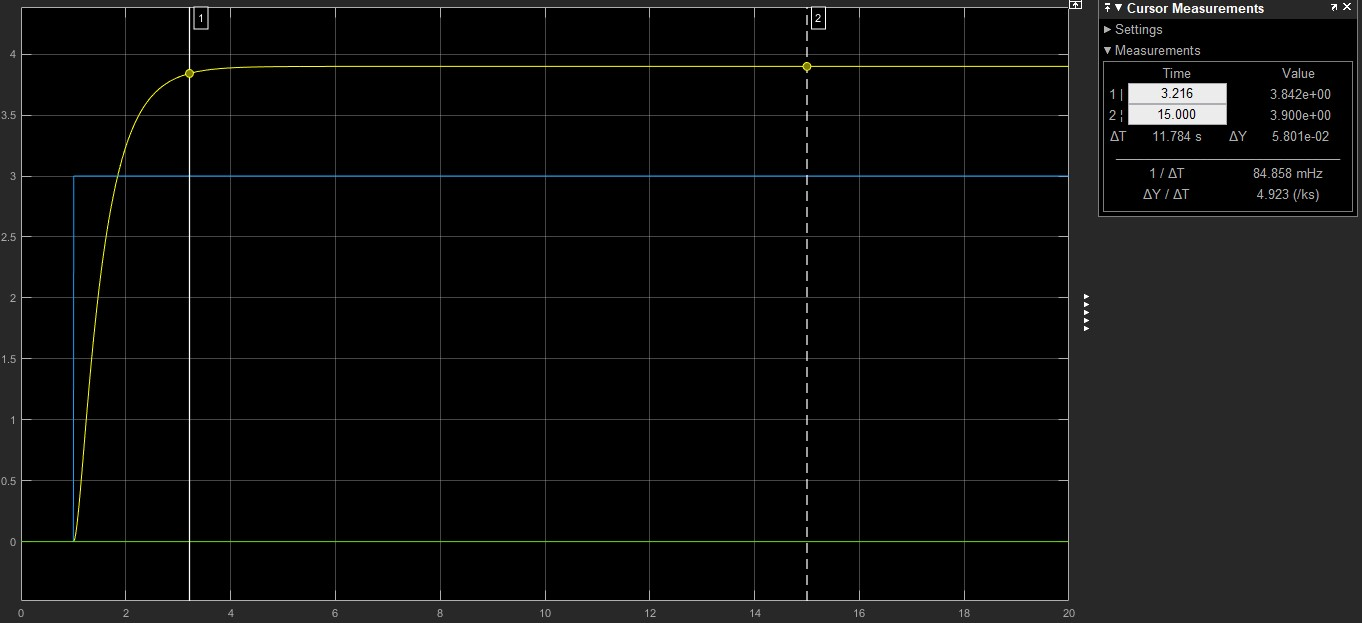
\includegraphics{Imagens/Lab3/Resolução/prob3AA.jpg}

Pela curva feita espera-se que a Função de Transferência seja de primeira ordem. Utilizando as ferramentas fornecidas pelo \texttt{Simulink} foi estimado que
\[
y(\infty) = 3.9 \\
0.95y(\infty) = 3.8415 \implies  t_s(5\%) = 3.22s \implies \tau = 1.072
\]

Assim,
\[
G_3(s) = \frac {1.3}{1.072s+1}.
\]

Simulando \(G_1(s)\), temos o resultado apresentado abaixo.

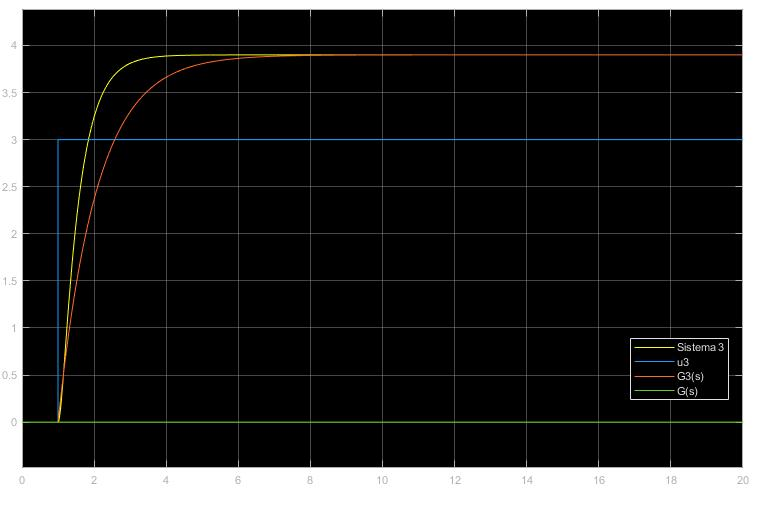
\includegraphics{Imagens/Lab3/Resolução/prob3AB.jpg}

Percebe-se, assim, que a Função de Transferência \(G_B(s)\) não se aproxima satisfatoriamente bem ao Sistema 3. Aplicando a malha fechada vista na figura 3, temos o resultado apresentado abaixo.

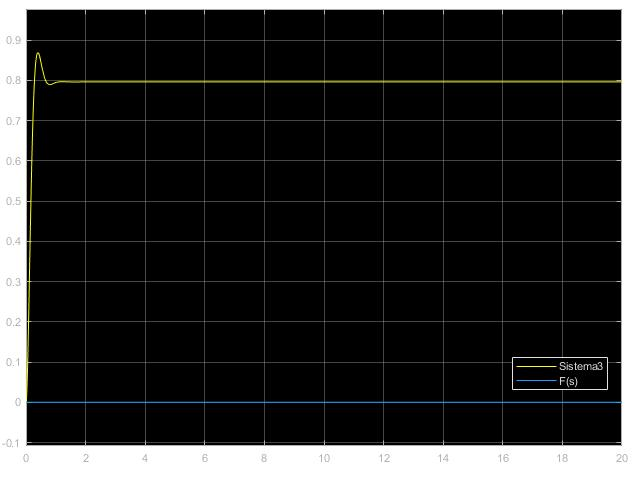
\includegraphics{Imagens/Lab3/Resolução/prob3AC.jpg}

Como \(K_c = 3 > 0\) e a Função de Transferência em malha fechada retornou um sistema de segunda ordem, percebe-se a resposta não está de acordo com a propriedade estabelecida. Desta forma, presume-se que \(G(s)\) não é de primeira ordem e sim de segunda.

\hypertarget{parte-b}{%
\subsubsection*{Parte B}\label{parte-b}}
\addcontentsline{toc}{subsubsection}{Parte B}

Identifique \(F(s)\). Em seguida, identifique \(G(s)\)indiretamente através da equação 3.5. Para isto, utilize os seguintes comandos no \texttt{Matlab}:

\begin{Shaded}
\begin{Highlighting}[]
\VariableTok{F} \OperatorTok{=} \VariableTok{tf}\NormalTok{([}\VariableTok{K}\OperatorTok{*}\VariableTok{wn}\OperatorTok{\^{}}\FloatTok{2}\NormalTok{]}\OperatorTok{,}\NormalTok{ [}\FloatTok{1} \FloatTok{2}\OperatorTok{*}\VariableTok{ksi}\OperatorTok{*}\VariableTok{wn} \VariableTok{wn}\OperatorTok{\^{}}\FloatTok{2}\NormalTok{])}
\VariableTok{G} \OperatorTok{=} \VariableTok{F}\OperatorTok{/}\NormalTok{(}\VariableTok{Kc}\OperatorTok{{-}}\VariableTok{Kc}\OperatorTok{*}\VariableTok{F}\NormalTok{)}
\VariableTok{G} \OperatorTok{=} \VariableTok{zpk}\NormalTok{(}\VariableTok{minreal}\NormalTok{(}\VariableTok{G}\NormalTok{)) }\CommentTok{\% minreal simplifica e zpk fatora}
\end{Highlighting}
\end{Shaded}

Note que \(G(s)\) é de segunda ordem com pólos reais. Neste momento, temos condições de responderm o que estava errado em nossa modelagem inicial do Sistema 3 como um sistema de primeira ordem. Compare a resposta em malha-aberta de \(G(s)\) (identificando indiretamente) com a do Sistema 3 para \(u(t) = 3\) do tipo degrau.

\hypertarget{resoluuxe7uxe3o-9}{%
\paragraph*{Resolução}\label{resoluuxe7uxe3o-9}}
\addcontentsline{toc}{paragraph}{Resolução}

Simulando o sistema do Sistema 3 em malha fechada e utilizando as ferramentas fornecidas pelo \texttt{Simulink} foi estimado que
\[
y_p = 0.868 \\
y(\infty) = 0.796 \\
t_p = 0.4s
\]

Assim, tem-se que:
\[
K = 0.796, \quad M_p = 0.09, \quad \xi = 0.61 \quad \text{e} \quad \omega_n= 9.888.
\]

Dessa forma, tem-se que
\[
F(s) = \frac {77.83}{s^2+ 12.01s +97.77}
\]
que gera a curva abaixo.

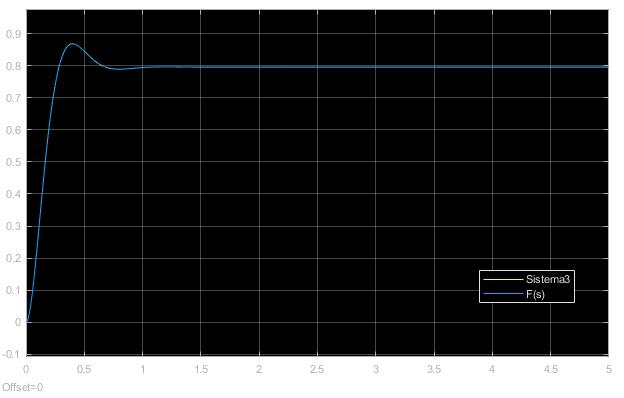
\includegraphics{Imagens/Lab3/Resolução/prob3BA.jpg}

Assim, é possível calcular \(G(s)\) a partir de \(F(s)\), tendo como resultado
\[
G(s) = \frac {25.94}{s^2+12.025s+19.96}.
\]

Agora é possível comprar \(G(s)\) com sua curva anterior, gerando o resultado abaixo.

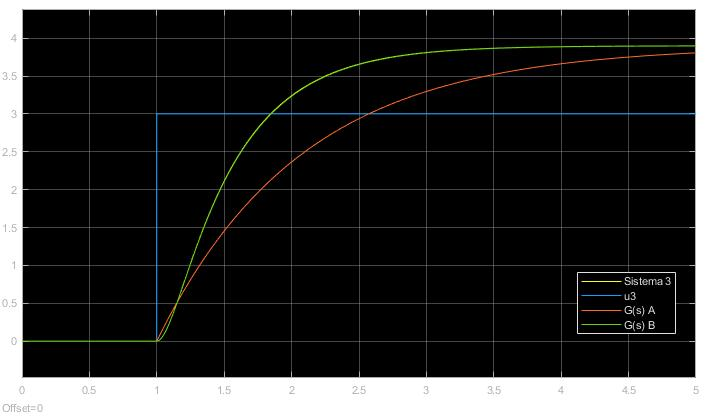
\includegraphics{Imagens/Lab3/Resolução/prob3BB.jpg}

Percebe-se que, considerando o modelo como uma Função de Transferência de segundo grau obtida através de \(F(s)\) é possível encontrar a curva exata correspondente ao Sistema 3.

\hypertarget{rastreamento-de-referuxeancias-e-rejeiuxe7uxe3o-de-perturbauxe7uxf5es---erro-em-regime-permanente}{%
\chapter{Rastreamento de Referências e Rejeição de Perturbações - Erro em Regime Permanente}\label{rastreamento-de-referuxeancias-e-rejeiuxe7uxe3o-de-perturbauxe7uxf5es---erro-em-regime-permanente}}

Working on it :)

\hypertarget{projeto-de-controladores-por-muxe9todos-alguxe9bricos}{%
\chapter{Projeto de Controladores por Métodos Algébricos}\label{projeto-de-controladores-por-muxe9todos-alguxe9bricos}}

Working on it :)

\hypertarget{linearizauxe7uxe3o-de-sistemas-nuxe3o-lineares}{%
\chapter{Linearização de Sistemas Não-Lineares}\label{linearizauxe7uxe3o-de-sistemas-nuxe3o-lineares}}

Working on it :)

\hypertarget{controle-de-sistemas-nuxe3o-lineares}{%
\chapter{Controle de Sistemas Não-Lineares}\label{controle-de-sistemas-nuxe3o-lineares}}

Working on it :)

\hypertarget{anuxe1lise-pelo-lugar-das-rauxedzes}{%
\chapter{Análise pelo Lugar das Raízes}\label{anuxe1lise-pelo-lugar-das-rauxedzes}}

Working on it :)

\hypertarget{projeto-de-controladores-pelo-lugar-das-rauxedzes}{%
\chapter{Projeto de Controladores pelo Lugar das Raízes}\label{projeto-de-controladores-pelo-lugar-das-rauxedzes}}

Working on it :)

\hypertarget{projeto-do-controlador-atraso-de-fase}{%
\chapter{Projeto do controlador atraso de fase}\label{projeto-do-controlador-atraso-de-fase}}

Working on it :)

\hypertarget{anuxe1lise-pelos-diagramas-de-bode-e-nyquist}{%
\chapter{Análise pelos Diagramas de Bode e Nyquist}\label{anuxe1lise-pelos-diagramas-de-bode-e-nyquist}}

Working on it :)

\hypertarget{projeto-de-controladores-pelo-diagrama-de-bode}{%
\chapter{Projeto de Controladores pelo Diagrama de Bode}\label{projeto-de-controladores-pelo-diagrama-de-bode}}

Working on it :)

\hypertarget{digitalizauxe7uxe3o-de-controladores-analuxf3gicos}{%
\chapter{Digitalização de Controladores Analógicos}\label{digitalizauxe7uxe3o-de-controladores-analuxf3gicos}}

Working on it :)

  \bibliography{book.bib,packages.bib}

\end{document}
